%
% Ricci-Krümmung
%
\section{Ricci-Krümmung
\label{buch:kruemmung:section:ricci}}
\kopfrechts{Ricci-Krümmung}
%
% fig-schnittkruemmung.tex
%
% (c) 2025 Prof Dr Andreas Müller
%
\begin{figure}
\centering
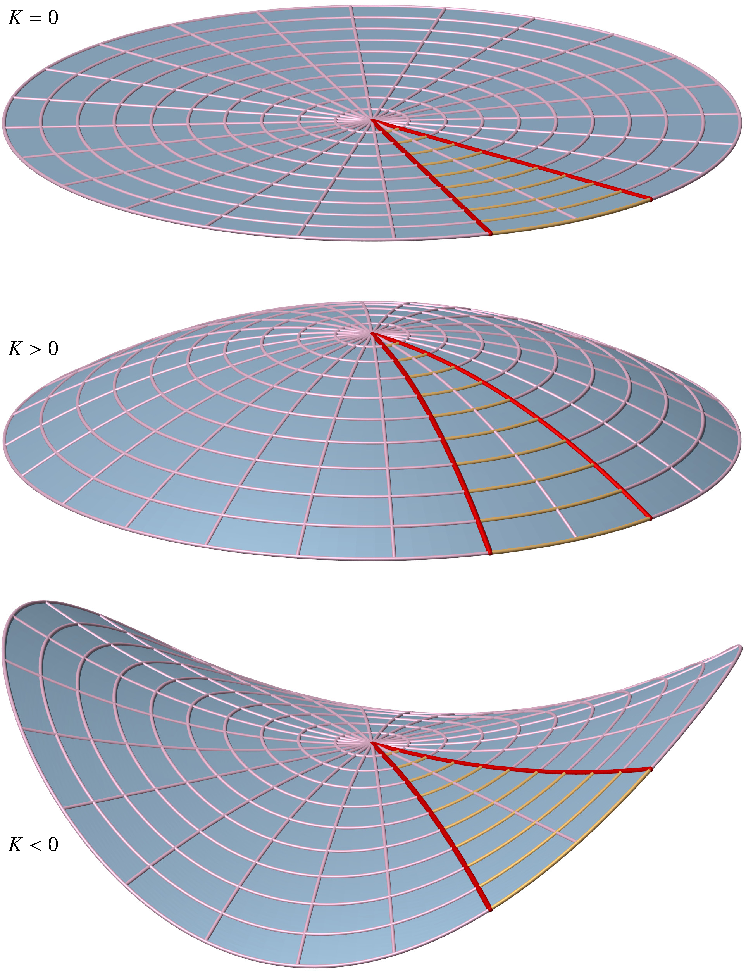
\includegraphics{chapters/110-kruemmung/images/kruemmung.pdf}
\caption{Die Schnittkrümmung bestimmt, wie schnell sich Geodäten
voneinander entfernen.
Der Abstand der Geodäten wächst linear mit dem Radius, wenn 
$K=0$ ist, der Abstand wächst schneller als linear für $K<0$ und
langsamer als linear für $K>0$.
\label{buch:kruemmung:fig:schnittkruemung}}
\end{figure}

Die Komponente $R^l\mathstrut_{ijk}$ des Riemann-Krümmungstensors
beschreibt, wie sich die $l$-Kom\-po\-nen\-te des $i$-ten 
Standardbasisvektors $\vec{e}_i$ beim Paralleltransport um
ein infinitesmales Quadrat mit dem 2-Vektor $\vec{e}_j\wedge \vec{e}_k$
verändert.
Für die physikalische Interpretation des Gravitationsfeldes ist
es wichtig zu verstehen, wie sich der Abstand von Geodäten mit
ähnlichen Anfangsbedingungen verändert, da wir dies als relative
Beschleunigung und damit als Anziehungs- oder Abstossungskraft 
interpretieren können.

%
% Der Ricci-Tensor
%
\subsection{Der Ricci-Tensor}
Der riemannsche Krümmungstensor wurde mit der linearen Abbildung
$R(X,Y)$ definiert, die ihrerseits durch
\[
R(X,Y)Z
=
\nabla_X\nabla_YZ - \nabla_Y\nabla_XZ-\nabla_{[X,Y]}Z
\]
definiert war.
Hält man $Y$ und $Z$ fest, ist $f:X\mapsto R(X,Y)Z$ eine lineare Abbildung.
Die Abbildung hängt ausserdem linear von den Vektoren $Y$ und $Z$ ab.

In einem Koordinatensystem $x^i$ ist die
Abbildung für $Y=\partial_k$ und $Z=\partial_l$  gegeben durch
\[
\partial_i
\mapsto
R(\partial_i,\partial_k)\partial_l
\]
Die Matrixelemente können daraus mithilfe des Skalarprodukts mit
einem Basisvektor ermittelt werden.
Die Basisvektoren werden gemäss
\[
\partial_i
\mapsto
\langle
R(\partial_i,\partial_k)\partial_l,
\partial_m
\rangle
=
R^{m}\mathstrut_{lik}\partial_m
\]
abgebildet.
Für die genannte spezielle Wahl von $Y$ und $Z$ sind also die 
die Matrixelemente von der Abbildung durch Komponenten des
riemannschen Krümmungstensors gegeben sind.
Die Matrix der Abbildung ist
\[
A^m\mathstrut_i
=
\begin{pmatrix}
R^1\mathstrut_{l1k} & R^1\mathstrut_{l2k} & \dots  & R^1\mathstrut_{lnk} \\
R^2\mathstrut_{l1k} & R^2\mathstrut_{l2k} & \dots  & R^2\mathstrut_{lnk} \\
\vdots              & \vdots              & \ddots & \vdots              \\
R^n\mathstrut_{l1k} & R^n\mathstrut_{l2k} & \dots  & R^n\mathstrut_{lnk} 
\end{pmatrix}.
\]
Um mehr über diese Abbildung zu erfahren, kann man bekannte
Invarianten linearer Abbildungen studieren.
Die Spur einer linearen Abbildung ist die Summe der Diagonalelemente,
also
\[
\operatorname{tr} A^m\mathstrut_i
=
\sum_{i=1}^n A^i\mathstrut_i.
\]
Es ist ein bekanntes Resultat der linearen Algebra, dass die Spur
unabhängig ist von der Wahl des Koordinatensystems.
Es folgt aus der Tatsache, dass ein Basiswechsel durch ein
Transformationsmatrix $T$ gegeben wird, mit der die Matrix der
Abbildung in der neuen Basis durch $A'=TAT^{-1}$ berechnet
werden kann.
Der Wert der Spur ist dann
\[
\operatorname{tr} A'
=
\operatorname{tr}(TAT^{-1})
=
\operatorname{tr}(A\underbrace{T^{-1}T}_{\displaystyle=I})
=
\operatorname{tr}A.
\]
Der Wert der Spur hängt also nicht von der Wahl der Basis ab.
Die Spur ist somit eine von der Wahl des Koordinatensystems
unabhängige Grösse, die bilinear von den Vektoren $Y$ und $Z$
abhängt.

\begin{definition}[Ricci-Tensor]
Der \emph{Ricci-Tensor} $Ric(Y,Z)$ ist die Spur der linearen Abbildung
\[
X \mapsto R(X,Y)Z = (\nabla_X\nabla_YZ-\nabla_Y\nabla_XZ-\nabla_{[X,Y]}Z.
\]
Für $Y=y^l\partial_l$ und $Z=z^k\partial_k$ ist der Wert der Spur
durch die Bilinearform
\[
Ric(Y,Z)
=
R^m\mathstrut_{lmk} y^lz^k
=
g^{im}
R_{ilmk}y^lz^k
\]
gegeben.
Die Komponenten des Ricci-Tensors sind also
\[
Ric(\partial_l,\partial_k)
=
R_{lk}
=
R^m\mathstrut_{lmk}
=
g^{im}
R_{ilmk}.
\]
\end{definition}

%
% Symmetrie
%
\subsubsection{Symmetrie}
Der Ricci-Tensor ist ein symmetrischer Tensor, wie man zum Beispiel
durch Anwendung der Symmetrieeigenschaften des riemannschen Krümmungstensors
in
\[
R_{kl}
=
g^{im}R_{ilmk}
=
g^{im}R_{mkil}
=
g^{im}R_{mkil}
=
g^{im}R_{ikml}
\]
sehen kann.
Im zweiten Schritt wurde die Symmetrie unter Vertauschung der beiden
Indexpaare verwendet, im dritten die Symmetrie des metrischen Tensors
und im letzten wurden die summierten Indizes umbenannt.

%
% Ricci-Tensor in Normalkoordinaten
%
\subsection{Ricci-Tensor in Normalkoordinaten}
In Normalkoordinaten kann man die Komponenten des Ricci-Tensors
nach \eqref{buch:kruemmung:kruemmung:eqn:Rruvm} im Punkt $p$ durch
\begin{align*}
R_{lk}
&=
g^{im}
R_{ilmk} 
\\
&=
\delta^{im}
\biggl(
\frac{\partial \Gamma^i_{lm}}{\partial x^k}
-
\frac{\partial \Gamma^i_{lk}}{\partial x^m}
\biggr)
\\
&=
\frac{\partial \Gamma^m_{lm}}{\partial x^k}
-
\frac{\partial \Gamma^m_{lk}}{\partial x^m}
\intertext{berechnen.
Da man ausserdem die Ableitungen der Christoffel-Symbole durch zweite
Ableitungen der metrischen Koeffizienten ausdrückenkann, kann man
den Ricci-Tensor mithilfe von \eqref{buch:kruemmung:kruemmung:eqn:Rddg}
auch als}
R_{lk}
&=
g^{im}
R_{ilmk} 
\\
&=
\delta^{im}
\frac12
\biggl(
\frac{\partial^2 g_{im}}{\partial x^k\,\partial x^l}
-
\frac{\partial^2 g_{lm}}{\partial x^k\,\partial x^i}
-
\frac{\partial^2 g_{ik}}{\partial x^m\,\partial x^l}
+
\frac{\partial^2 g_{lk}}{\partial x^m\,\partial x^i}
\biggr)
\\
&=
\frac12
\sum_{m=1}^n
\biggl(
\frac{\partial^2 g_{mm}}{\partial x^k\,\partial x^l}
-
\frac{\partial^2 g_{lm}}{\partial x^k\,\partial x^m}
-
\frac{\partial^2 g_{mk}}{\partial x^m\,\partial x^l}
+
\frac{\partial^2 g_{lk}}{\partial (x^m)^2}
\biggr)
\end{align*}
schreiben.
Der letzte Term dieses Ausdrucks erinnert an den Laplace-Operator,
angewendet auf alle Komponenten.

Tatsächlich ist eine Anwendung des Ricci-Tensors die Definition einer
Differentialgleichung für den metrischen Tensor auf einer riemannsche
Mannigfaltigkeit, die der Wärmeleitung ähnlich ist.
Die Zeitentwicklung der Lösung, der sogenannte Ricci-Fluss, deformiert
die Metrik derart, dass die Krümmung reduziert wird, so wie die
Wärmeleitungsgleichung die Temperaturverteilung glättet.
Mit diesem Werkzeug wurde es möglich, die Poincaré-Vermutung, eines
der berühmten Millenniumsprobleme, zu lösen.

%
% Krümmungsskalar
%
\subsection{Krümmungsskalar}
Die Spur des Ricci-Tensors 
\[
S
=
g^{ik}R_{ik}
=
R^i_k
\]
ist ebenfalls eine koordinatensystemunabhängige Grösse, sie
heisst der {\em Krümmungsskalar}.
\index{Krummungsskalar@Krümmungsskalar}
Der Krümmungsskalar ist als Tensor nullter Stufe eine weitere Invariante,
die in einer Feldgleichung für die Gravitation vorkommen könnte.

Der Tensor $Sg$ mit den Komponenten $Sg_{ik}$ hat die Spur
\[
\operatorname{tr} Sg
=
Sg^{ik}g_{ik}
=
nS.
\]
Daher ist $\frac1n Sg$ ein symmetrischer Tensor mit der gleichen
Spur wie der Ricci-Tensor. 
Wir bezeichnen mit
\[
\overset{\circ}{Ric}
=
Ric - \frac1n Sg
\]
den \emph{spurlosen Ricci-Tensor}.

Die besondere Bedeutung des Krümmungsskalars ist, dass die Zerlegung
\begin{equation}
Ric
=
\overset{\circ}{Ric} + \frac1n Sg
\label{buch:kruemmung:ricci:eqn:Riczerlegung}
\end{equation}
orthogonal ist.

\begin{satz}
Die Zerlegung \eqref{buch:kruemmung:ricci:eqn:Riczerlegung} ist
orthogonal, d.~h.~der spurlose Ricci-Tensor $\overset{\circ}{Ric}$
und $\frac1nSg$ sind orthogonal.
\end{satz}

\begin{proof}
Sei $h$ ein beliebiger symmetrischer Tensor mit Komponenten $h_{ik}$,
dann ist das Skalarprodukt mit dem metrischen Tensor mit den 
Komponenten $g_{lm}$ durch
\begin{align*}
\langle h,g\rangle
&=
h_{ik}g_{lm}
g^{il}g^{km}
=
h_{ik}\delta_m^i
g^{km}
=
h_{ik}g^{ik}
=
\operatorname{tr} h
\end{align*}
gegeben.
Daher ist das Skalarprodukt
\[
\langle \overset{\circ}{Ric},\frac{1}n Sg \rangle
=
\frac1nS\langle\overset{\circ}{Ric},g\rangle
=
\frac1nS\operatorname{tr}\overset{\circ}{Ric}
=
0,
\]
die Tensoren $\overset{\circ}{Ric}$ und $\frac1nSg$ sind orthogonal.
\end{proof}

Die äussere Ableitung des Krümmungsskalars kann durch Kontraktion
der kovarianten Ableitung des Ricci-Tensors gewonnen werden.

%
% Kontrahierte Bianchi-Identitäten
%
\subsection{Kontrahierte Bianchi-Identitäten}
Der Ricci-Tensor entsteht durch Kontraktion zweier Indizes aus dem
riemannschen Krümmungstensor gewonnen.
Die Bianchi-Identitäten müssen sich daher auch in Identitäten
für den Ricci-Tensor äussern.
Wir berechnen diese Identitäten zunächst in Komponenten, bevor wir
eine koordinatenfreie Beschreibung geben.

%
% Kontrahierte algebraische Bianchi-Identität
%
\subsubsection{Kontrahierte algebraische Bianchi-Identität}
Die algebraische Bianchi-Identität besagt, dass
\[
0
=
R_{iklm}
+
R_{ilmk}
+
R_{imkl}.
\]
Multiplikation mit $g^{il}$ wird daraus
\begin{align*}
0
&=
R_{km}
+
g^{il}R_{ilmk}
+
g^{il}R_{imkl}.
\intertext{Der mittlere Term verschwindet, weil der riemannsche
Krümmungstensor in den ersten beiden Indizes $il$ antisymmetrisch ist,
während $g^{il}$ symmetrisch ist.
Im letzten Term können wir die letzten zwei Indizes vertauschen, was
das Vorzeichen kehrt.
So entsteht}
&=
R_{km}
-
g^{il}R_{imlk}
\\
&=
R_{km}-R_{mk}.
\end{align*}
Die erste Bianchi-Identität liefert also nichts anderes als die
Symmetrie des Ricci-Tensors, die wir bereits kennen.

%
% Kontrahierte differentielle Bianchi-Identität
%
\subsubsection{Kontrahierte differentielle Bianchi-Identität}
Wir wenden die Kontraktion auch auf die differentielle Bianchi-Identität
\[
0
=
R_{abik;l}
+
R_{abkl;i}
+
R_{abli;k}
\]
an und erhalten
\begin{align}
0
&=
g^{ai}
(
R_{abik;l}
+
R_{abkl;i}
+
R_{abli;k}
)
\notag
\\
&=
R_{bk;l}
+
g^{ai}
R_{abkl;i}
+
g^{ai}
R_{abli;k}
\notag
\\
&=
R_{bk;l}
+
g^{ai}
R_{abkl;i}
-
g^{ai}
R_{abil;k}
\notag
\\
&=
R_{bk;l}
+
g^{ai}
R_{abkl;i}
-
R_{bl;k}
\notag
\\
R^i\mathstrut_{bkl;i}
&=
-(
R_{bk;l}
-
R_{bl;k}
).
\label{buch:kruemmung:ricci:eqn:kontrdbianchi}
\end{align}
Die Formel \eqref{buch:kruemmung:ricci:eqn:kontrdbianchi} kann
man noch in eine koordinatenfreie Form bringen und damit besser
verstehen.
Hält man in $\textit{Ric}(X,Y)$ einen der Vektor fest,
entsteht eine $1$-Form.
Der Ricci-Tensor kann also als eine 1-Form mit Werten in 
1-Formen betrachten.
Wir schreiben $\boldsymbol{\alpha}$ für die 1-Form $X\mapsto R(X,Y)$
und berechnen die kovariante äussere Ableitung.
Sie erfüllt
\begin{align*}
\langle \boldsymbol{d}\boldsymbol{\alpha}, Y\wedge Z\rangle
&=
\nabla_Y\langle\boldsymbol{\alpha},Z\rangle
-
\nabla_Z\langle\boldsymbol{\alpha},Y\rangle
-
\langle \boldsymbol{\alpha}, [Y,Z] \rangle
\intertext{Auf dem Vektor $X$ hat diese 1-Form den Wert}
\langle\boldsymbol{d}\boldsymbol{\alpha},Y\wedge Z\rangle (X)
&=
\nabla_Y {Ric}(X,Z)
-
\nabla_Z {Ric}(X,Y)
-
{Ric}(X,[Y,Z])
\end{align*}
Setzt man für die Vektoren $X$, $Y$ und $Z$ die Standardbasisvektoren
$\partial_b$, $\partial_k$ und $\partial_l$ ein, wird daraus
\begin{align*}
\langle\boldsymbol{d}\boldsymbol{\alpha},\partial_k\wedge \partial_l\rangle
(\partial_b)
&=
\nabla_k {Ric}(\partial_b,\partial_l)
-
\nabla_l {Ric}(\partial_b,\partial_k)
-
{Ric}(\partial_b,[\partial_k,\partial_l]).
\intertext{Weil die Basisoperatoren $\partial_i$ vertauschen ist
$[\partial_k,\partial_l])=0$ und der letzte Term fällt weg.
Es bleibt}
&=
\nabla_k {Ric}(\partial_b,\partial_l)
-
\nabla_l {Ric}(\partial_b,\partial_k)
=
R_{bl;k}
-
R_{bk;l}
\end{align*}
Die kontrahierte differentielle Bianchi-Identität sagt also, dass
die Spur der kovarianten Ableitung des riemannschen Krümmungstensors
die kovariante äussere Ableitung des Ricci-Tensors ist.

%
% Kontrahierte Bianchi-Identität und Krümmungsskalar
%
\subsubsection{Kontrahierte Bianchi-Identität und Krümmungsskalar}
Wir könnten von der kontrahierten Bianchi-Identität für den Ricci-Tensor
ausgehen, es ist aber etwa gleich einfach, die wieder von der differentiellen
Bianchi-Identität für den riemannschen Krümmungstensor auszugehen.
Damit lassen sich die Symmetrien des riemannschen Krümmungstensors etwas
offensichtlicher ausnützen.
Wir beginnen mit der Identität
\eqref{buch:kruemmung:kruemmung:eqn:diffbianchikomp},
die wir in der Form
\[
R_{abmn;l}
+
R_{ablm;n}
+
R_{abnl;m}
=
0
\]
schreiben.
Jetzt kontrahieren wir die Indexpaare $a$,$m$ und $b$,$n$ und erhalten
\begin{align}
g^{am}g^{bn}
(
R_{abmn;l}
+
R_{ablm;n}
+
R_{abnl;m}
)
&=
0.
\notag
\intertext{Die Kontraktion mit $g^{am}$ hebt den ersten Index dies
Riemannschen Krümmungstensors an:}
g^{bn}(
R^m\mathstrut_{bmn;l}
+
R^m\mathstrut_{blm;n}
+
R^m\mathstrut_{bnl;m}
)
&=
0.
\notag
\intertext{Im zweiten Term können wir die Indizes $l$ und $m$ vertauschen,
was zu einem Vorzeichenwechsel führt:}
g^{bn}(
R^m\mathstrut_{bmn;l}
-
R^m\mathstrut_{bml;n}
+
R^m\mathstrut_{bnl;m}
)
&=
0.
\notag
\intertext{Die ersten beiden Terme sind jetzt als kovariante Ableitungen
des Ricci-Tensors erkennbar. 
Im dritten Term können wir die Indizes $m$ und $b$ vertauschen, was
einen Vorzeichenwechsel zur Folge hat:}
g^{bn}(
R_{bn;l}
-
R_{bl;n}
-
R_b\mathstrut^m\mathstrut_{nl;m}
)
&=
0.
\notag
\intertext{Die Multiplikation mit $g^{bn}$ macht aus dem unteren
Index $b$ einen oberen Index $n$:}
R^n\mathstrut_{n;l}
-
R^n\mathstrut_{l;n}
-
R^{nm}\mathstrut_{nl;m}
&=
0.
\notag
\intertext{Der erste Term ist die Ableitung des Krümmungsskalars.
Auch der letzte Term als jetzt als kovariante Ableitung
des Ricci-Tensors erkennbar:}
S_{;l}
-
R^n\mathstrut_{l;n}
-
R^{m}\mathstrut_{l;m}
&=
0.
\notag
\intertext{Die letzten beiden Terme sind dasselbe, da sie sich nur
in der Bezeichnung für den Summationsindex unterscheiden.
Es folgt}
S_{;l}
&=
2
R^n\mathstrut_{l;n}
\notag
\intertext{oder}
R^n\mathstrut_{l;n}
&=
\frac12 S.
\label{buch:kruemmung:eqn:kontrahiertS}
\end{align}
Dies ist die kontrahierte Bianchi-Identität für den Krümmungsskalar.




